\documentclass[12pt]{article}
\usepackage[margin=1in]{geometry}
\usepackage[utf8]{inputenc}
\usepackage[spanish]{babel}
\usepackage{parskip}
\usepackage{setspace}
\usepackage{amsmath, amssymb}
\usepackage{graphicx}
\usepackage{tikz}
\usepackage{hyperref} % Siempre debe ir al final.

% Opciones de Paquetes.
\decimalpoint           % {babel}
\onehalfspacing         % {setspace}
\usetikzlibrary{babel}  % {tikz}
\graphicspath{{./img/}} % {graphics}

% Encabezado.
\title{Clase 9. Aplicaciones de la derivada parcial: Aproximación lineal y optimización.}
\author{MIT 18.02: Multivariable Calculus.}
\date{}


\begin{document}

% Comandos personalizados.
%=========================================
%
%    Comandos personalizados usados en
%       los apuntes de este curso.
%
%=========================================

\newcommand{\vecmat}[1]{\mathbf{#1}}                          % Vectores o matrices en negrita en math mode.
\newcommand{\unitvec}[1]{\vecmat{\hat{#1}}}                   % Vectores unitarios.
\newcommand{\overvec}[1]{\overrightarrow{#1}}                 % Vector como segmento orientado.
\newcommand{\proy}[2]{\text{proy}_{\vecmat{#2}}{\vecmat{#1}}} % Proyección vectorial.
\newcommand{\invmat}[1]{\vecmat{#1}^{-1}}                     % Inversa de una matriz.
\newcommand{\transmat}[1]{\vecmat{#1}^{T}}                    % Transpuesta de una matriz.
\newcommand{\Adj}[0]{\text{Adj}}                              % Matriz adjunta.
\newcommand{\R}[0]{\mathbb{R}}                                % Símbolo conjunto de los números reales.
\newcommand{\N}[0]{\mathbb{N}}                                % Símbolo conjunto de los números naturales.


\maketitle

\begin{abstract}
\noindent Similar a su par ordinaria, con la derivada parcial es posible obtener aproximaciones lineales en un punto de la función multivariada original, así como evaluar y (si existen) encontrar los valores máximos, mínimos y/o de ensillado de esta última. Es por ello que esta clase se centra en estudiar dichas aplicaciones de la diferenciación parcial.
\end{abstract}


\section{Aproximación lineal y diferenciabilidad.}

Cuando una función $f(x)$ es diferenciable en $x = x_{0}$, es posible observar en un plano cartesiano que su curva irá asemejándose a la recta tangente que pasa por ese punto a medida que se acorta el eje horizontal a valores cercanos a $x_{0}$, cuya ecuación corresponde a la aproximación lineal de $f$ en $x_{0}$. En esta sección estudiamos lo mismo, pero para funciones multivariadas y, con ella, también definiremos su diferenciabilidad.

\subsection{Ecuación del plano tangente.}

Sean $z = f(x, \ y)$, $f_{x}$ y $f_{y}$ una función junto con sus primeras derivadas parciales, todas caracterizadas por ser \textbf{continuas}. Además, asumamos que tanto $f_{x}(x_{0}, \ y_{0})$ como $f_{y}(x_{0}, \ y_{0})$ existen, con $(x_{0}, \ y_{0})$ siendo un par ordenado del dominio de $z$.

Dado que $f_{x}(x_{0}, \ y_{0})$ y $f_{x}(x_{0}, \ y_{0})$ existen, podemos considerarlas como las pendientes de dos rectas tangentes que se intersectan en la superficie de $z$ en el punto $(x_{0}, \ y_{0}, \ z_{0})$. Como se ve en la siguiente imagen, mediante ambas figuras es posible formar un plano.

\newpage

\begin{figure}[hbt!]
\centering
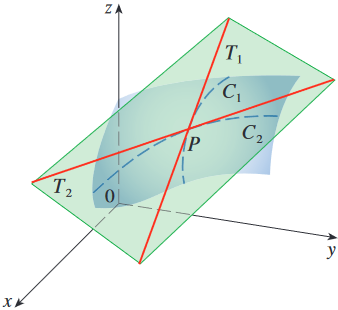
\includegraphics[scale=0.48]{plano-tangente.png}
\caption{Stewart, et al (2021). \textit{Calculus. Early Transcendentals. Metric Version}. Pp. 974}
\end{figure}

En la imagen de arriba, $P$ es el punto $(x_{0}, \ y_{0}, \ z_{0})$ de la superficie de $z$. Las figuras $C_{1}$ y $C_{2}$ son las curvas generadas al cortar a $z$ mediante los planos $y = y_{0}$ y $x = x_{0}$, respectivamente; mientras que $T_{1}$ y $T_{2}$ son las rectas tangentes a $C_{1}$ y $C_{2}$ en $P$. A partir de $T_{1}$ y $T_{2}$ se forma el llamado \textbf{plano tangente} a la superficie de $z$ en $P$.

La ecuación del plano tangente a $z$ en $P$ la podemos buscar a partir de la siguiente igualdad que estudiamos en la Clase 4:\footnote{En esa ocasión la llamamos como la ecuación cartesiana del plano.}
\[
  A(x - x_{0}) + B(y - y_{0}) + C(z - z_{0}) = D
\]
Asumamos que $C \neq 0$ y que $D = 0$. Esto implica que:
\[
  A(x - x_{0}) + B(y - y_{0}) + C(z - z_{0}) = 0
\]
A partir de los supuestos señalados arriba, dividamos esta ecuación por $C$.
\[
  \frac{A}{C}(x - x_{0}) + \frac{B}{C}(y - y_{0}) + z - z_{0} = 0
\]
Luego, despejemos a $z - z_{0}$ y establezcamos que $a = -A/C$ y $b = -B/C$.
\[
  z - z_{0} = a(x - x_{0}) + b(y - y_{0})
\]
Si $y = y_{0}$, obtenemos la ecuación de una recta $z = f(x, \ y_{0})$ en forma punto-pendiente.
\[
  z - z_{0} = a(x - x_{0})
\]
Recordemos que $y = y_{0}$ es el plano que corta a la superficie de $z$ en $P$ a lo largo de $x$. Por lo tanto, la igualdad de arriba corresponde a la ecuación de la recta tangente en $P$ de la curva que se forma en $y = y_{0}$ y, como consecuencia, podemos asumir que $a = f_{x}(x_{0}, \ y_{0})$.
\[
  z - z_{0} = f_{x}(x_{0}, \ y_{0}) \cdot (x - x_{0})
\]
Siguiendo la misma lógica que conllevó a la igualdad de arriba, si $x = x_{0}$, entonces:
\[
  z - z_{0} = b(y - y_{0})
\]
implicando que $b = f_{y}(x_{0}, \ y_{0})$ y, por consiguiente, que:
\[
  z - z_{0} = f_{y}(x_{0}, \ y_{0}) \cdot (y - y_{0})
\]
La ecuación $z - z_{0} = a(x - x_{0}) + b(y - y_{0})$ proviene de calcular la ecuación del plano tangente de $z$ en $P$, que es formado por las dos rectas tangentes que se intersectan en $P$. Por lo tanto, es posible establecer que $a = f_{x}(x_{0}, \ y_{0})$ y $b = f_{y}(x_{0}, \ y_{0})$ en esta igualdad, conllevando a que:
\[
  z - z_{0} = f_{x}(x_{0}, \ y_{0}) (x - x_{0}) + f_{y}(x_{0}, \ y_{0}) (y - y_{0})
\]
La igualdad de arriba recibe el nombre de \textbf{ecuación del plano tangente} a $z$ en $P$. Dado que $z = f(x, \ y)$, esta igualdad también puede ser expresada como:
\[
  f(x, \ y) - f(x_{0}, \ y_{0}) = f_{x}(x_{0}, \ y_{0}) (x - x_{0}) + f_{y}(x_{0}, \ y_{0}) (y - y_{0})
\]

\subsection{Aproximación lineal de una función multivariada.}

Calculemos la ecuación del plano tangente de la función $f(x, \ y) = 2x^{2} + y^{2}$ en el punto $(1, \ 1, \ 3)$. Para ello, comencemos con $f_{x}(x, \ y)$ y $f_{y}(x, \ y)$ en $(1, \ 1)$.
\begin{align*}
f_{x}(x, \ y) &= 4x & f_{y}(x, \ y) &= 2y \\
\therefore f_{x}(1, \ 1) &= 4 & \therefore f_{y}(1, \ 1) &= 2
\end{align*}
Como $f(1, \ 1) = 3$, entonces la ecuación del plano tangente a $f(x, \ y)$ en $(1, \ 1, \ 3)$ es:
\[
  f(x, \ y) - 3 = 4(x - 1) + 2(y - 1)
\]
Ahora resolvamos los productos del lado derecho de la ecuación de arriba.
\[
  f(x, \ y) - 3 = 4x + 2y - 6
\]
Si despejamos a $f(x, \ y)$ en la ecuación de arriba, sería incorrecto expresarla como una igualdad porque $f(x, \ y) = 2x^{2} + y^{2}$. En realidad, lo que se obtiene es la aproximación lineal de esta función cerca de $(1, \ 1)$.
\[
  f(x, \ y) \approx 4x - 2y - 3
\]
La expresión del lado derecho de esta aproximación corresponde a la linealización de $f(x, \ y)$ en $(1, \ 1)$ y se suele denotar como $L(x, \ y)$.
\[
  L(x, \ y) = 4x - 2y - 3
\]
Geométricamente, $L(x, \ y)$ corresponde al plano tangente de $f(x, \ y)$ en $(1, \ 1, \ 3)$.

La intuición geométrica de la aproximación lineal que acabamos de ver es que, a medida que acercamos los intervalos de los ejes $x$ e $y$ del espacio euclidiano al punto $(1, \ 1)$, la superficie de $f(x, \ y)$ irá asemejándose cada vez más a su plano tangente $L(x, \ y)$ en ese lugar, como se observa en la imagen de a continuación.

\begin{figure}[hbt!]
\centering
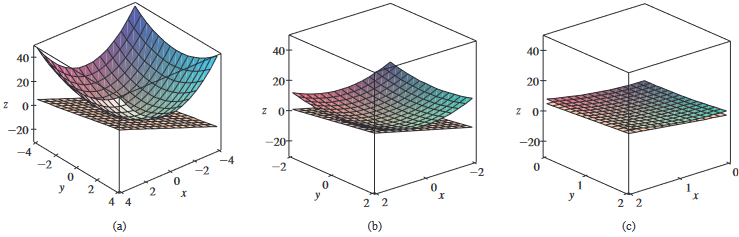
\includegraphics[scale=0.55]{aprox-lineal.png}
\caption{Stewart, et al (2021). \textit{Calculus. Early Transcendentals. Metric Version}. Pp. 975}
\end{figure}

Generalicemos lo visto hasta ahora. Considere la ecuación del plano tangente en $(x_{0}, \ y_{0}, \ z_{0})$ vista al final de la sección 1.1.
\[
  f(x, \ y) - f(x_{0}, \ y_{0}) = f_{x}(x_{0}, \ y_{0}) (x - x_{0}) + f_{y}(x_{0}, \ y_{0}) (y - y_{0})
\]
Al despejar a $f(x, \ y)$ se obtiene la \textbf{aproximación lineal} de $f(x, \ y)$ en $(x_{0}, \ y_{0})$.
\[
  f(x, \ y) \approx f(x_{0}, \ y_{0}) + f_{x}(x_{0}, \ y_{0}) (x - x_{0}) + f_{y}(x_{0}, \ y_{0}) (y - y_{0})
\]
Y se define a la siguiente función $L(x, \ y)$ como la \textbf{linealización} de $f(x, \ y)$ en $(x_{0}, \ y_{0})$.
\[
  L(x, \ y) = f(x_{0}, \ y_{0}) + f_{x}(x_{0}, \ y_{0}) (x - x_{0}) + f_{y}(x_{0}, \ y_{0}) (y - y_{0})
\]
Así, $L(x, \ y)$ es la mejor aproximación a $f(x, \ y)$ cuando $(x, \ y)$ es cercano a $(x_{0}, \ y_{0})$.\footnote{La precisión de $L(x, \ y)$ disminuye a medida que $(x, \ y)$ toma valores alejados de $(x_{0}, \ y_{0})$.}

\subsection{Diferenciabilidad de una función multivariada.}

Una función univariada $f(x)$ es diferenciable en un punto si su primera derivada existe en ese lugar. Cuando se cumple aquello, también se puede concluir que es continua en dicha ubicación. En el caso de las multivariadas, su diferenciabilidad no se puede garantizar de la misma manera.

Por ejemplo, considere la siguiente función:
\[
f(x, \ y) =
\left\{
\begin{aligned}
  \frac{xy}{x^{2} + y^{2}} \quad \text{ si } (x, \ y) \neq (0, \ 0) \\
  0 \quad \text{ si } (x, \ y) = (0, \ 0)
\end{aligned}
\right.
\]
Primero veamos si $f_{x}(0, \ 0)$ y $f_{y}(0, \ 0)$ existen usando sus definiciones del límite.
\begin{align*}
  f_{x}(0, \ 0) &= \lim_{\Delta x \to 0} \frac{f(0 + \Delta x, \ 0) - f(0, \ 0)}{\Delta x}
                 = \lim_{\Delta x \to 0} \frac{f(\Delta x, \ 0) - 0}{\Delta x} \\
  f_{y}(0, \ 0) &= \lim_{\Delta y \to 0} \frac{f(0, \ 0 + \Delta y) - f(0, \ 0)}{\Delta y}
                 = \lim_{\Delta y \to 0} \frac{f(0, \ \Delta y) - 0}{\Delta y}
\end{align*}
Asumiendo que tanto $\Delta x$ como $\Delta y$ no son iguales a cero, entonces:
\[
  f(\Delta x, \ 0) = \frac{\Delta x \cdot 0}{(\Delta x)^{2} + 0^{2}} = 0 \qquad \qquad
  f(0, \ \Delta y) = \frac{0 \cdot \Delta y}{0^{2} + (\Delta y)^{2}} = 0
\]
Mediante lo anterior se puede concluir que tanto $f_{x}(0, \ 0)$ como $f_{y}(0, \ 0)$ existen y son iguales a cero.
\begin{align*}
  f_{x}(0, \ 0) &= \lim_{\Delta x \to 0} \frac{0}{\Delta x} = \lim_{\Delta x \to 0} 0 = 0 &
  f_{y}(0, \ 0) &= \lim_{\Delta y \to 0} \frac{0}{\Delta y} = \lim_{\Delta y \to 0} 0 = 0
\end{align*}
Ahora evaluemos el límite de $f(x, \ y)$ a medida que $(x, \ y)$ se acerca al origen a lo largo de $y = x$.
\[
\limbiv{0, \ 0} f(x, \ x) = \limbiv{0, \ 0} \frac{x \cdot x}{x^{2} + x^{2}}
                          = \limbiv{0, \ 0} \frac{x^{2}}{2x^{2}}
                          = \limbiv{0, \ 0} \frac{1}{2}
                          = \frac{1}{2}
\]
Lo anterior implica que en $y = x$:
\[
  \limbiv{0, \ 0} f(x, \ y) \neq f(0, \ 0)
\]
Esto significa que $f(x, \ y)$ no es continua en $(0, \ 0)$.

El ejemplo anterior muestra la dificultad de determinar la diferenciabilidad de una función de varias variables: Que $f_{x}(0, \ 0)$ y $f_{y}(0, \ 0)$ existan no determina que $f(x, \ y)$ sea continua en su origen. Por este motivo, nos ayudaremos de una propiedad que puede obtenerse en funciones de una variable para evaluar esta característica en las multivariadas.

Sea $L(x) = f(x_{0}) + f'(x_{0})(x - x_{0})$ la linealización de $f(x)$ en $x = x_{0}$. El error de la aproximación lineal de $f(x)$ en $x = x_{0} + \Delta x$ puede medirse como:
\[
  \text{error apróx} = \Delta f - \Delta L
\]
Donde $\Delta f = f(x_{0} + \Delta x) - f(x_{0})$, mientras que $\Delta L$ es:
\[
  \Delta L = L(x_{0} + \Delta x) - L(x_{0})
           = f'(x_{0}) \Delta x
\]
De este modo,
\[
  \text{error apróx} = f(x_{0} + \Delta x) - f(x_{0}) - f'(x_{0}) \Delta x
                     = \left(\frac{f(x_{0} + \Delta x) - f(x_{0})}{\Delta x} - f'(x_{0})\right) \Delta x
\]
Si establecemos que:
\[
  \epsilon = \frac{f(x_{0} + \Delta x) - f(x_{0})}{\Delta x} - f'(x_{0})
\]
Entonces,
\[
  \text{error apróx} = \epsilon \Delta x
\]
Observemos, por una parte, que:
\[
  \lim_{\Delta x \to 0} \epsilon = \lim_{\Delta x \to 0} \left(\frac{f(x_{0} + \Delta x) - f(x_{0})}{\Delta x} - f'(x_{0})\right)
                                 = f'(x_{0}) - f'(x_{0})
                                 = 0
\]
Y, por otra parte, que al despejar a $f(x_{0} + \Delta x) - f(x_{0}) = \Delta f$ en la definición de $\epsilon$ se obtiene:
\[
  \Delta f = f'(x_{0}) \Delta x + \epsilon \Delta x
\]
Al tomar el límite a medida que $\Delta x \to 0$ en la igualdad de arriba, $\Delta f$ resulta aproximadamente en:
\[
  \lim_{\Delta x \to 0} \Delta f = f'(x_{0}) \Delta x = \Delta L
\]
puesto que $\epsilon \to 0$ cuando $\Delta x \to 0$, lo que implica que $\epsilon \Delta x \to 0$ en ese contexto. Con esto, se puede concluir que $L(x)$ será una buena aproximación de $f(x)$ en $x = x_{0}$ cuando esta función es diferenciable en ese punto. Usaremos esta propiedad para definir la diferenciabilidad de funciones de varias variables.

Sea $z = f(x, \ y)$ una función bivariada y $\Delta z$ el valor de su cambio desde $(x_{0}, \ y_{0})$ hasta $(x_{0} + \Delta x, \ y_{0} + \Delta y)$.
\[
  \Delta z = f(x_{0} + \Delta x, \ y_{0} + \Delta y) - f(x_{0}, \ y_{0})
\]
Definiremos que $z = f(x, \ y)$ es \textbf{diferenciable} en $(x_{0}, \ y_{0})$ si $\Delta z$ puede ser expresada como:
\[
  \Delta z = f_{x}(x_{0}, \ y_{0}) \Delta x + f_{y}(x_{0}, \ y_{0}) \Delta y + \epsilon_{x} \Delta x + \epsilon_{y} \Delta y
\]
donde $\epsilon_{x} \to 0$ y $\epsilon_{y} \to 0$ a medida $(\Delta x, \ \Delta y) \to (0, \ 0)$.

Esta definición de la diferenciabilidad de $z = f(x, \ y)$ se vincula con la calidad de su aproximación lineal en $(x, \ y) = (x_{0}, \ y_{0})$. Primero veamos que:
\[
  \Delta L = L(x_{0} + \Delta x, \ y_{0} + \Delta y) - L(x_{0}, \ y_{0})= f_{x}(x_{0}, \ y_{0}) \Delta x + f_{y}(x_{0}, \ y_{0}) \Delta y
\]
En ese sentido, cuando $\Delta z$ puede ser expresada como en la definición de la diferenciabilidad de $z$, implicando que $\lim_{\Delta x \to 0} \epsilon_{x} = 0$ y $\lim_{\Delta y \to 0} \epsilon_{y} = 0$, entonces:
\[
  \Delta z \approx \Delta L
\]
Es decir, cuando $z = f(x, \ y)$ es diferenciable en $(x_{0}, \ y_{0})$, su plano tangente en ese lugar dada por $L(x, \ y)$ es una buena aproximación a $z$ en ese punto, donde $\epsilon_{x} \Delta x$ y $\epsilon_{y} \Delta y$ son los errores de las aproximaciones lineales de las funciones univariadas $f(x, \ y_{0})$ en $x = x_{0} + \Delta x$ y $f(x_{0}, \ y)$ en $y = y_{0} + \Delta y$, respectivamente.

De la definición de diferenciabilidad de $z = f(x, \ y)$ en $(x_{0}, \ y_{0})$ se desprenden los siguientes dos teoremas:

\textbf{Teorema 1.} Si las derivadas parciales $f_{x}$ y $f_{y}$ de $f(x, \ y)$ existen y son continuas en $(x_{0}, \ y_{0})$, entonces $f(x, \ y)$ es \textbf{diferenciable} en $(x_{0}, \ y_{0})$.

\textbf{Teorema 2.} Si $f(x, \ y)$ es diferenciable en $(x_{0}, \ y_{0})$, entonces es \textbf{continua} en $(x_{0}, \ y_{0})$.

El Teorema 1 también puede aplicarse a toda la región abierta de $z = f(x, \ y)$.\footnote{Si $f_{x}$ y $f_{y}$ existen y son continuas a lo largo de una región abierta $R$ de $f(x, \ y)$, entonces dicha función es diferenciable en cada punto donde está definida.} Su idea detrás es que cuando esta función es diferenciable en un punto o en todo su dominio, se puede asegurar que $\Delta z \to 0$ cuando $\Delta x \to 0$ y $\Delta y \to 0$, con $\Delta z = f(x_{0} + \Delta x, \ y_{0} + \Delta y) - f(x_{0}, \ y_{0})$.

Por otra parte, el Teorema 2 formaliza a partir de la definición de diferenciabilidad que dicha característica en $z = f(x, \ y)$ permite asegurar que es continua en ese lugar (o en todo su dominio).

\ejemplo Demuestre que $f(x, \ y) = x \cdot \exp(xy)$ es diferenciable en $(1, \ 0)$. Luego, calcule su linealización en ese punto y utilícela para aproximar el valor $f(1.1, \ -0.1)$.

\solucion Comencemos calculando las primeras derivadas parciales de $f(x, \ y)$, donde la expresión $\exp(xy) = (\exp(x))^{y} = (\exp(y))^{x}$.
\begin{align*}
\derivpar{x} (x \cdot (\exp(x))^{y}) &= \exp(xy) + xy (\exp(x))^{y - 1} \exp(x) = \exp(xy) + xy \exp(xy) \\
\derivpar{y} (x \cdot (\exp(y))^{x}) &= x \cdot \derivpar{y} (\exp(y))^{x} = x^{2} \exp(xy)
\end{align*}
Podemos dar por hecho que tanto $f_{x} = \exp(xy) + xy \exp(xy)$ como $f_{y} = x^{2} \exp(xy)$ son funciones continuas. Además, están definidas en el punto $(1, \ 0)$, como se ve a continuación.
\begin{align*}
 \pderivpar{x}{(x \cdot \exp(xy))}{(1, \ 0)} &= \exp(1 \cdot 0) + (1 \cdot 0) \exp(1 \cdot 0) = 1 \\
 \pderivpar{y}{(x \cdot \exp(xy))}{(1, \ 0)} &= 1^{2} \exp(1 \cdot 0) = 1
\end{align*}
Así, por el Teorema 1, $f(x, \ y)$ es diferenciable en el punto $(1, \ 0)$.

Busquemos la linealización de $f(x, \ y)$ en $(1, \ 0)$.
\[
  L(x, \ y) = (1 \cdot \exp(1 \cdot 0)) + f_{x}(1, \ 0)(x - 1) + f_{y}(1, \ 0)(y - 0)
            = x + y
\]
Luego, evaluemos a $L(x, \ y) = x + y$ en $(1.1, \ -0.1)$.
\[
  L(1.1, \ -0.1) = 1.1 + (-0.1) = 1
\]
El resultado de arriba indica que el valor de $f(x, \ y) = x \cdot \exp(xy)$ en $(1.1, \ -0.1)$ se aproxima a $1$. De hecho, usando una calculadora podemos ver que $f(1.1, \ -0.1) \approx 0.9854$.


\section{Optimización: Valores extremos y puntos de silla de una función.}

Mediante las primeras y segundas derivadas parciales de una función multivariada se pueden conocer sus valores extremos (locales o globales) bajo supuestos similares a los usados con funciones univariadas. Sin embargo, a diferencia de estas últimas, en las primeras también es posible encontrar otro punto crítico conocido como punto de silla (\textit{saddle point}). Todo esto lo estudiamos en esta sección.

\subsection{Valores extremos locales.}

Sea $f(x, \ y)$ una función definida en una región $R$ y considere un punto $(x_{0}, \ y_{0}) \in R$. Para todo $(x, \ y)$ miembro de un disco abierto con centro en $(x_{0}, \ y_{0})$, se señala que:

\begin{itemize}
\item $f(x_{0}, \ y_{0})$ es un valor \textbf{máximo local} de $f$ si $f(x, \ y) \leq f(x_{0}, \ y_{0})$.

\item $f(x_{0}, \ y_{0})$ es un valor \textbf{mínimo local} de $f$ si $f(x, \ y) \geq f(x_{0}, \ y_{0})$.
\end{itemize}

Los dos $f(x_{0}, \ y_{0})$ vistos arriba, en conjunto, se conocen como \textbf{valores extremos locales} (o extremos relativos). La palabra \textit{local} se debe a que son máximos o mínimos dentro de un conjunto\footnote{La subregión de $R$ que corresponde al disco abierto centrado en $(x_{0}, \ y_{0})$.} de valores $(x, \ y)$ cercanos a $(x_{0}, \ y_{0})$.

En las secciones que siguen veremos cómo determinar los extremos locales mediante las pruebas de las primeras y segundas derivadas parciales de $f(x, \ y)$.

\subsection{Prueba de las primeras derivadas y los puntos críticos.}

Una manera de evaluar si $f(x_{0}, \ y_{0})$ es un extremo local, es a partir de la \textbf{prueba de las primeras derivadas} de $f$. Esta indica que $f(x_{0}, \ y_{0})$ es un valor máximo o mínimo local si:

\begin{enumerate}
\item Tanto $f_{x}$ como $f_{y}$ existen en $(x_{0}, \ y_{0})$.
\item $f_{x}(x_{0}, \ y_{0}) = f_{y}(x_{0}, \ y_{0}) = 0$
\end{enumerate}

La explicación geométrica de esta prueba es que, cuando se cumplen las dos condiciones de arriba, el plano tangente a $f(x, \ y)$ en $(x_{0}, \ y_{0})$ es horizontal. Aquello se puede apreciar en la ecuación de esta superficie ya que se iguala a una función constante.
\[
  f(x, \ y) - f(x_{0}, \ y_{0}) = 0 + 0 \Longrightarrow f(x, \ y) = f(x_{0}, \ y_{0})
\]
Cuando se cumple una de las siguientes condiciones:

\begin{enumerate}
\item $f_{x}(x_{0}, \ y_{0}) = f_{y}(x_{0}, \ y_{0}) = 0$ 
\item $f_{x}$ o $f_{y}$ o ambas no están definidas en $(x_{0}, \ y_{0})$.
\end{enumerate}

se señala que $(x_{0}, \ y_{0})$ es un \textbf{punto crítico} de la función $f(x, \ y)$.

Por lo tanto, si se cumple la \textbf{prueba de las primeras derivadas parciales} de $f(x, \ y)$ en $(x_{0}, \ y_{0})$, se puede concluir que $(x_{0}, \ y_{0})$ es un \textbf{punto crítico} de $f$. Más específicamente, recibe el nombre de \textbf{punto estacionario} de $f$.

En cambio, cuando $f_{x}(x_{0}, \ y_{0})$ o $f_{y}(x_{0}, \ y_{0})$ o ambas no están definidas, entonces $(x_{0}, \ y_{0})$ se llama \textbf{punto singular} de $f$.

\subsection{Punto de silla.}

Al saber que $(x_{0}, \ y_{0})$ es un punto crítico de $f(x, \ y)$ porque $f_{x}(x_{0}, \ y_{0}) = f_{y}(x_{0}, \ y_{0}) = 0$, significa que el valor $f(x_{0}, \ y_{0})$ puede ser una de las tres siguientes opciones:

\begin{enumerate}
\item Un máximo local (o global) de $f(x, \ y)$.
\item Un mínimo local (o global) de $f(x, \ y)$.
\item Ni un máximo ni un mínimo local de $f(x, \ y)$.
\end{enumerate}

Cuando ocurre la tercera opción señalada arriba, entonces es posible que $(x_{0}, \ y_{0})$ sea un \textbf{punto de silla} (\textit{saddle point}) de $f$.

Sea $f:R \to \R$, con $R \subseteq \R^{2}$, una función diferenciable en $(x_{0}, \ y_{0}) \in R$, donde este par ordenado es el centro de un disco abierto $D \subset R$. Se dice que $(x_{0}, \ y_{0})$ es un \textbf{punto de silla} de $f$ si:

\begin{itemize}
\item Es un punto crítico (estacionario) de $f$.
\item Para algunos $(x, \ y) \in D$, $f(x, \ y) < f(x_{0}, \ y_{0})$.
\item Y para otros $(x, \ y) \in D$, $f(x, \ y) > f(x_{0}, \ y_{0})$.
\end{itemize}

\ejemplo Busque (si es que existen) los extremos locales de las funciones:
\[
  \text{(a) } f(x, \ y) = y^{2} - x^{2} \qquad \qquad
  \text{(b) } g(x, \ y) = x^{2} + y^{3}
\]
\solucion Comencemos buscando los puntos críticos de $f(x, \ y)$ y $g(x, \ y)$. Para ello, calculemos sus primeras derivadas parciales:
\begin{align*}
  f_{x} &= -2x & f_{y} &= 2y \\
  g_{x} &= 2x  & g_{y} &= 3y^{2}
\end{align*}
Luego, busquemos las raíces de las derivadas parciales de arriba.
\begin{align*}
f_{x} &= 0  &  f_{y} &= 0  &  g_{x} &= 0  &   g_{y} &= 0 \\
  -2x &= 0  &     2y &= 0  &     2x &= 0  &  3y^{2} &= 0 \\
    x &= 0  &      y &= 0  &      x &= 0  &       y &= 0
\end{align*}
Así, dado que se cumple la prueba de las primeras derivadas parciales en $f(x, \ y)$ y $g(x, \ y)$, podemos concluir que $(0, \ 0)$ es un punto estacionario de ambas funciones.

Evaluemos el punto $(0, \ 0)$ a lo largo de $x$ y de $y$ tanto en $f(x, \ y)$ como en $g(x, \ y)$.
\begin{align*}
  f(x, \ 0) &= -x^{2} & f(0, \ y) &= y^{2} \\
  g(x, \ 0) &= x^{2}  & g(0, \ y) &= y^{3}
\end{align*}
A partir de las igualdades de arriba se tiene, por una parte, que:
\[
  \forall x \in \R; \; f(x, \ 0) < 0 \qquad \qquad
  \forall y \in \R; \; f(0, \ y) > 0
\]
Mientras que, por otra parte,
\[
  \forall x \in \R; \; g(x, \ 0) > 0 \qquad
  \forall y \in \R^{+}; \; g(0, \ y) > 0 \qquad
  \forall y \in R^{-}; \; g(0, \ y) < 0
\]
Es decir, $(0, \ 0)$ es un punto de silla tanto en $f(x, \ y)$ como en $g(x, \ y)$ porque, en ambas funciones, no son ni un máximo ni un mínimo local a pesar de ser un punto estacionario.

En el ejemplo que acabamos de resolver vimos dos tipos de punto de silla. En $f(x, \ y) = y^{2} - x^{2}$ se observó que a lo largo de $x$, $f(0, \ 0)$ corresponde a un máximo local, mientras que en la trayectoria de $y$ es un mínimo local. Por otra parte, en $g(x, \ y) = x^{2} + y^{3}$, $g(0, \ 0)$ a lo largo de $x$ es un mínimo local, pero en la trayectoria de $y$ dicho valor no es un máximo ni un mínimo\footnote{En este caso, $(0, \ 0)$ corresponde a un \textbf{punto de inflexión} de la curva $g(0, \ y)$, que es donde su segunda derivada ordinaria (y, por tanto, su curvatura) cambia de signo.}.

\subsection{Prueba de las segundas derivadas.}

Cuando se cumple la prueba de las primeras derivadas parciales en $f(x, \ y)$, solo tenemos certeza de que existe un extremo local, pero no si es un máximo, mínimo o si es solo un punto de silla. Para determinar a estos últimos, se debe aplicar la prueba de las segundas derivadas parciales de $f$.

Sea $f\colon R \to \R$, con $R \subseteq \R^{2}$, una función y $f_{x}$, $f_{y}$, $f_{xx}$, $f_{xy}$, $f_{yx}$ y $f_{yy}$ sus derivadas parciales definidas en $R$ y, junto con $f$, \textbf{continuas} en $(x_{0}, \ y_{0}) \in R$. Luego, considere la siguiente matriz $\vecmat{H}$ de las segundas derivadas parciales de $f$ en $(x_{0}, \ y_{0})$, conocida como \textbf{matriz hessiana}.
\[
\vecmat{H} =
\begin{bmatrix}
f_{xx}(x_{0}, \ y_{0}) & f_{xy}(x_{0}, \ y_{0}) \\
f_{yx}(x_{0}, \ y_{0}) & f_{yy}(x_{0}, \ y_{0})
\end{bmatrix}
\]
Por las características de $f$ así como de sus segundas derivadas parciales, se cumple por el teorema de Clairaut que $f_{xy} = f_{yx}$. De este modo, el $\det(\vecmat{H})$ (o determinante hessiano) está dado por:
\[
  \det(\vecmat{H}) = f_{xx}(x_{0}, \ y_{0}) f_{yy}(x_{0}, \ y_{0}) - (f_{xy}(x_{0}, \ y_{0}))^{2}
\]
Usaremos el $\det(\vecmat{H})$ para definir la \textbf{prueba de las segundas derivadas} de $f$, la que señala que si esta función y sus (primeras y segundas) derivadas parciales son continuas a lo largo de un disco $D \subset R$ con centro en $(x_{0}, \ y_{0})$ y si $f_{x}(x_{0}, \ y_{0}) = f_{y}(x_{0}, \ y_{0}) = 0$, entonces:

\begin{enumerate}
\item $f(x_{0}, \ y_{0})$ es un \textbf{mínimo local} de $f$ cuando $f_{xx}(x_{0}, \ y_{0}) < 0$ y $\det(\vecmat{H}) > 0$.
\item $f(x_{0}, \ y_{0})$ es un \textbf{máximo local} de $f$ cuando $f_{xx}(x_{0}, \ y_{0}) > 0$ y $\det(\vecmat{H}) > 0$.
\item $f(x_{0}, \ y_{0})$ es un \textbf{punto de silla} de $f$ cuando $\det(\vecmat{H}) < 0$.
\item La prueba \textbf{no es concluyente} en $(x_{0}, \ y_{0})$ si $\det(\vecmat{H}) = 0$.
\end{enumerate}

Cuando es usado en la prueba de las segundas derivadas parciales de $f$, el $\det(\vecmat{H})$ suele ser mencionado como \textbf{discriminante}.

\ejemplo Busque los puntos críticos de $f(x, \ y) = 10xy \exp(-x^{2} - y^{2})$ y clasifíquelos como mínimos locales, máximos locales o puntos de silla a partir de lo que obtenga al aplicar la prueba de las segundas derivadas parciales de $f$ en esos lugares.

\solucion Comencemos calculando las primeras derivadas parciales de $f$.
\begin{align*}
  \derivpar{x}{f} &= 10y \cdot \derivpar{x} (x \cdot \exp(-x^{2} - y^{2}))
                   = 10y (1 - 2x^{2}) \exp(-x^{2} - y^{2}) \\ \\
  \derivpar{y}{f} &= 10x \cdot \derivpar{y} (y \cdot \exp(-x^{2} - y^{2}))
                   = 10x (1 - 2y^{2}) \exp(-x^{2} - y^{2})
\end{align*}
Tanto $f_{x}$ como $f_{y}$ son funciones continuas a lo largo del dominio (o región) de $f$. Por lo tanto, los puntos críticos de $f$ son estacionarios y podemos buscarlos a partir de la prueba de las primeras derivadas parciales.
\begin{align*}
\derivpar{x}{f} &= 0 & \derivpar{y}{f} &= 0 \\
10y(1 - 2x^{2}) \exp(-x^{2} - y^{2}) &= 0 & 10x(1 - 2y^{2}) \exp(-x^{2} - y^{2}) &= 0
\end{align*}
Un primer punto estacionario que se obtiene de las dos ecuaciones de arriba, es $(0, \ 0)$. El resto de ellos pueden encontrarse al despejar a $(1 - 2x^{2})$ en la igualdad de la izquierda y a $(1 - 2y^{2})$ en la de la derecha.
\begin{align*}
1 - 2x^{2} &= 0 & 1 - 2y^{2} &= 0 \\
x &= \pm \frac{1}{\sqrt{2}} & y &= \pm \frac{1}{\sqrt{2}}
\end{align*}
En síntesis, los puntos estacionarios de $f$ son:
\[
  (0, \ 0) \qquad (1/\sqrt{2}, \ 1/\sqrt{2}) \qquad (-1/\sqrt{2}, \ 1/\sqrt{2}) \qquad
  (1/\sqrt{2}, \ -1/\sqrt{2}) \qquad (-1/\sqrt{2}, \ -1/\sqrt{2})
\]
Continuemos calculando las segundas derivadas parciales de $f$.
\begin{align*}
       \nderivpar{2}{x}f &= \derivpar{x}[10y (1 - 2x^{2}) \exp(-x^{2} - y^{2})]
                          = -20xy (3 - 2x^{2}) \exp(-x^{2} - y^{2}) \\ \\
       \nderivpar{2}{y}f &= \derivpar{x}[10x (1 - 2y^{2}) \exp(-x^{2} - y^{2})]
                          = -20xy (3 - 2y^{2}) \exp(-x^{2} - y^{2}) \\ \\
  \nbiderivpar{2}{x}{y}f &= \derivpar{y}[10y (1 - 2x^{2}) \exp(-x^{2} - y^{2})]
                          = 10 (1 - 2x^{2}) (1 - 2y^{2}) \exp(-x^{2} - y^{2})
\end{align*}
Al calcular $f_{yx}$ veremos que $f_{xy} = f_{yx}$, lo que se condice con el teorema de Clairaut porque $f$ y sus primeras y segundas derivadas parciales son todas continuas a lo largo del dominio de esta función.

Luego de conocer las segundas derivadas parciales de $f$, solo resta aplicar la prueba de las segundas derivadas en cada punto estacionario de $f$. Los resultados de este proceso se resumen en la siguiente tabla\footnote{Los resultados numéricos se pueden ver al ejecutar en R el script \texttt{\href{run:scripts/ejemplo-3.R}{ejemplo-3.R}} que está en la carpeta \texttt{scripts}.}.

\begin{table}[hbt!]
\centering
\renewcommand{\arraystretch}{1.5}

\begin{tabular}{c c c}
\hline
      Ptos. estacionarios      & $f_{xx}(x_{0}, \ y_{0})$ & $\det(\vecmat{H})$ \\
\hline
         $(0, \ 0)$            &              $= 0$       &        $< 0$       \\
$(1/\sqrt{2}, \ 1/\sqrt{2})$   &              $< 0$       &        $> 0$       \\
$(-1/\sqrt{2}, \ 1/\sqrt{2})$  &              $> 0$       &        $> 0$       \\
$(1/\sqrt{2}, \ -1/\sqrt{2})$  &              $> 0$       &        $> 0$       \\
$(-1/\sqrt{2}, \ -1/\sqrt{2})$ &              $< 0$       &        $> 0$       \\
\hline
\end{tabular}

\end{table}

De la tabla de arriba se puede concluir que:

\begin{itemize}
\item $(0, \ 0)$ es un punto de silla de $f$.
\item $f(1/\sqrt{2}, \ 1/\sqrt{2})$ y $f(-1/\sqrt{2}, \ -1/\sqrt{2})$ son mínimos locales de $f$.
\item $f(-1/\sqrt{2}, \ 1/\sqrt{2})$ y $f(1/\sqrt{2}, \ -1/\sqrt{2})$ son máximos locales de $f$.
\end{itemize}

\subsection{Valores extremos absolutos.}

La búsqueda de los valores extremos de una función se puede extender a todo su dominio y no solo a un subconjunto de este. Aquellos reciben la etiqueta de \textit{absolutos} o \textit{globales}.

Considere una función $f \colon R \to \R$ ($R \subseteq \R^{2}$) y un par ordenado $(x_{0}, \ y_{0}) \in R$. Entonces:

\begin{itemize}
\item $f(x_{0}, \ y_{0})$ es un valor \textbf{máximo absoluto} de $f$ en $R$ si $f(x_{0}, \ y_{0}) \geq f(x, \ y)$ $\forall (x, \ y) \in R$.
\item $f(x_{0}, \ y_{0})$ es un valor \textbf{mínimo absoluto} de $f$ en $R$ si $f(x_{0}, \ y_{0}) \leq f(x, \ y)$ $\forall (x, \ y) \in R$.
\end{itemize}

Para buscar los extremos absolutos de $f$ debemos:

\begin{enumerate}
\item Buscar sus puntos críticos en $R$ y evaluar el valor que toma en esas ubicaciones.
\item Buscar sus valores extremos en la frontera de $R$.
\end{enumerate}

El valor \textbf{más grande} de $f$ que se obtiene en los dos pasos de arriba será el \textbf{máximo absoluto}, mientras que el \textbf{más pequeño} será el \textbf{mínimo absoluto}.

\ejemplo Encuentre los extremos absolutos de la función $f(x, \ y) = x^{2} - 2xy + 2y$ en la región rectangular $R = \{(x, \ y) \ | \ 0 \leq x \leq 3, \ 0 \leq y \leq 2\}$.

\solucion  Comencemos calculando las derivadas parciales de $f(x, \ y)$.
\[
  f_{x}(x, \ y) = 2x - 2y = 2(x - y) \qquad f_{y}(x, \ y) = -2x + 2 = -2(x - 1)
\]
Luego, busquemos los puntos críticos de $f(x, \ y)$ mediante las raíces de sus primeras derivadas parciales.
\begin{align*}
f_{x}(x, \ y) &= 0 & f_{y}(x, \ y) &= 0 \\
2(x - y) &= 0 & -2(x - 1) &= 0 \\
y &= x & x &= 1
\end{align*}
Observemos que $f_{x}(x, \ y) = 0$ si $y = x$, mientras que $f_{y}(x, \ y) = 0$ cuando $x = 1$. Por lo tanto, solo es posible que $f_{x} = f_{y} = 0$ cuando $(x, \ y) = (1, \ 1)$. De este modo, se puede concluir que dicho par ordenado es un \textbf{punto estacionario} de $f(x, \ y)$, donde $f(1, \ 1) = 1$.

Ahora veamos qué valores toma $f(x, \ y)$ en la frontera de la región rectangular $R$. Esta puede ser representada mediante cuatro segmentos que denotaremos como $L_{1}$, $L_{2}$, $L_{3}$ y $L_{4}$.

\begin{figure}[hbt!]
\centering

\begin{tikzpicture}
%\draw[help lines] (-0.5, -0.5) grid (6, 6);

\draw[-latex, line width = 0.3mm] (0, 0) -- (5, 0) node [right] {$x$};
\draw[-latex, line width = 0.3mm] (0, 0) -- (0, 4) node [above] {$y$};

\draw[color=black!30!green, fill=green!30, line width=0.5mm] (0,0) rectangle (4, 3);

\node at (2, 1.5) {$R$};

\foreach \x \i in {-0.6/0, 4/3} {
  \node[font=\small] at (\x, 3.3) {$(\i, \ 2)$};
  \node[font=\small] at (\x, -0.3) {$(\i, \ 0)$};
}

\foreach \i \j in {1/-0.3, 3/3.3} {
  \node[font = \small] at (2, \j) {$L_{\i}$};
}

\foreach \i \j in {2/4.3, 4/-0.3} {
  \node[font = \small] at (\j, 1.5) {$L_{\i}$};
}

\end{tikzpicture}

\end{figure}

De este modo, para cada uno de los cuatro segmentos vistos en la figura de arriba podemos obtener las siguientes funciones que provienen de $f(x, \ y)$:

\begin{table}[hbt!]
\centering

\begin{tabular}{c c c}
Segmento & $f(x, \ y)$ & Dominio \\
\hline
$L_{1}$ & $f(x, \ 0) = x^{2}$ & $0 \leq x \leq 3$ \\
$L_{2}$ & $f(3, \ y) = 9 - 4y$ & $0 \leq y \leq 2$ \\
$L_{3}$ & $f(x, \ 2) = x^{2} - 4x + 4$ & $0 \leq x \leq 3$ \\
$L_{4}$ & $f(0, \ y) = 2y$ & $0 \leq y \leq 2$
\end{tabular}

\end{table}

Evaluemos a las funciones de $L_{1}$, $L_{2}$, $L_{3}$ y $L_{4}$ en sus respectivas \textbf{fronteras} (i.e, en los límites de sus dominios).

\begin{table}[hbt!]
\centering

\begin{tabular}{c c c}
Segmento & Límite inferior & Límite superior \\
\hline
$L_{1}$ & $f(0, \ 0) = 0$ & $f(3, \ 0) = 9$ \\
$L_{2}$ & $f(3, \ 0) = 9$ & $f(3, \ 2) = 1$ \\
$L_{3}$ & $f(0, \ 2) = 4$ & $f(3, \ 2) = 1$ \\
$L_{4}$ & $f(0, \ 0) = 0$ & $f(0, \ 2) = 4$
\end{tabular}

\end{table}

Así, los puntos donde es posible encontrar los extremos absolutos de $f(x, \ y)$ son:

\begin{table}[hbt!]
\centering

\begin{tabular}{c l}
Par ordenado & Característica \\
\hline
$(1, \ 1)$ & Punto estacionario \\
$(0, \ 0)$ & Frontera \\
$(3, \ 0)$ & Frontera \\
$(0, \ 2)$ & Frontera
\end{tabular}

\end{table}

Cabe agregar que en $L_{3}$, $f(x, \ 2) = x^{2} - 4x + 4 = (x - 2)^{2}$. Esto implica que $f(2, \ 2) = 0$. Es decir, dicho valor también es un candidato a ser un extremo absoluto de $f(x, \ y)$.

Al estudiar a $f(x, \ y) = x^{2} - 2xy + 2y$ en su punto crítico y en los de frontera, se puede concluir que $f(0, \ 0) = f(2, \ 2)$ es su mínimo absoluto y $f(3, \ 2)$ su máximo absoluto.

\end{document}